%&latex
\documentclass{article}

\usepackage{tikz}
\usetikzlibrary{chains}

\begin{document}

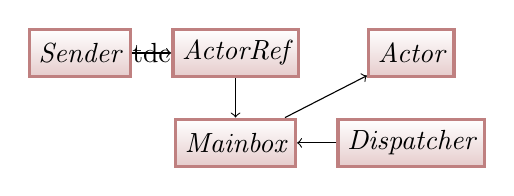
\begin{tikzpicture}[node distance=5mm,
	nonterminal/.style={
		% The shape:
		rectangle,
		% The size:
		minimum size=6mm,
		% The border:
		very thick,
		draw=red!50!black!50, % 50% red and 50% black,
		% and that mixed with 50% white
		% The filling:
		top color=white, % a shading that is white at the top...
		bottom color=red!50!black!20, % and something else at the bottom
		% Font
		font=\itshape
		}]

	\node (sender) [nonterminal] {Sender};
	\node (actorref) [nonterminal,right=of sender] {ActorRef};
	\node (mailbox) [nonterminal,below=of actorref] {Mainbox};
	\node (dispatcher) [nonterminal,right=of mailbox] {Dispatcher};
	\node (actor) [nonterminal,above=of dispatcher] {Actor};

	\path (sender) edge[->] node {tdc} (actorref); % simple edges
	\path (actorref) edge[->] (mailbox); % simple edges
	\path (dispatcher) edge[->] (mailbox); % simple edges
	\path (mailbox) edge[->] (actor); % simple edges

\end{tikzpicture}

\end{document}


